\documentclass{article}
\usepackage{ctex}

% Set page size and margins
% Replace `letterpaper' with `a4paper' for UK/EU standard size
\usepackage[letterpaper,top=2cm,bottom=2cm,left=2.5cm,right=2.5cm,marginparwidth=1.75cm]{geometry}

% Useful packages
\usepackage{amsmath}
\usepackage{graphicx}
\usepackage{subfigure}
\usepackage{float}
\usepackage[colorlinks=true, allcolors=blue]{hyperref}

\title{微分方程数值解计算实习课后作业12}
\author{陈文宇}
\date{\today}


\begin{document}


\maketitle

\tableofcontents

\newpage
%---------------------------------------------------
\section{实验结果}

下图是三种格式的数值解和精确解的图像,三种格式的结果基本相同,仅给出一组结果.
\begin{figure}[H]
\subfigure[正视图]{
\begin{minipage}[t]{0.45\linewidth}
\centering
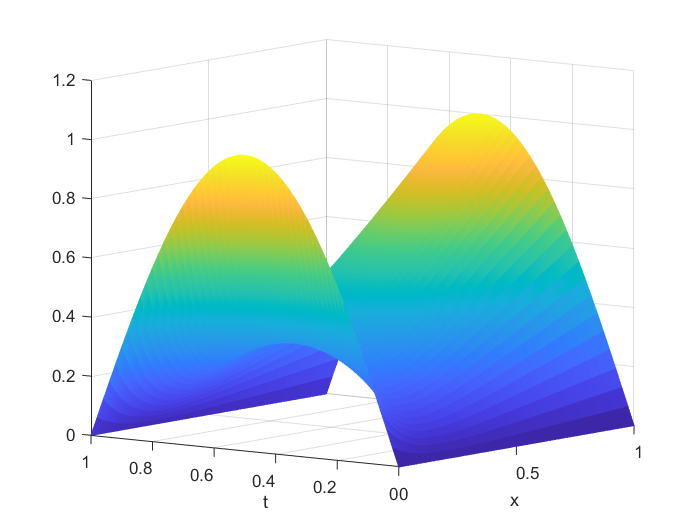
\includegraphics[scale=0.4]{solution_front.png}
\end{minipage}
}
\subfigure[侧视图]{
\begin{minipage}[t]{0.45\linewidth}
\centering
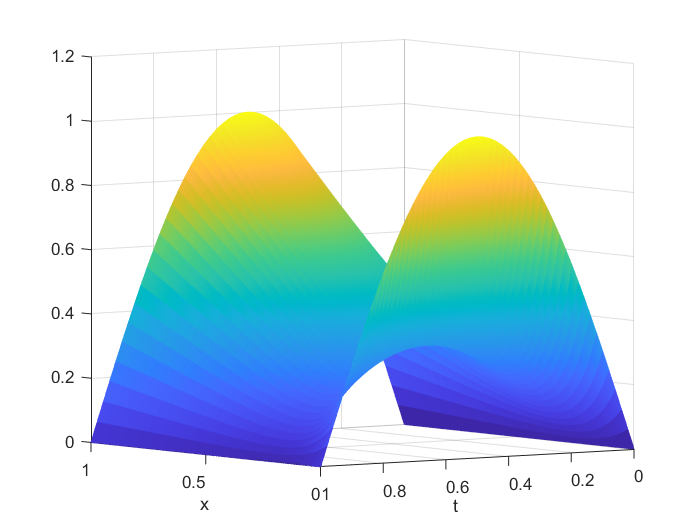
\includegraphics[scale=0.4]{solution_side.png}
\end{minipage}
}
\caption{\label{solution_image}数值解和精确解的图像}
\end{figure}

下图是$(logh,log(err0))$的图像,同$y=h^2$,$y=t $对比知,err0 误差关于h的收敛阶为2,关于t的收敛阶为1.
三种格式的结果基本相同,仅给出一组结果.
\begin{figure}[H]
	\subfigure{
		\begin{minipage}[t]{0.45\linewidth}
			\centering
			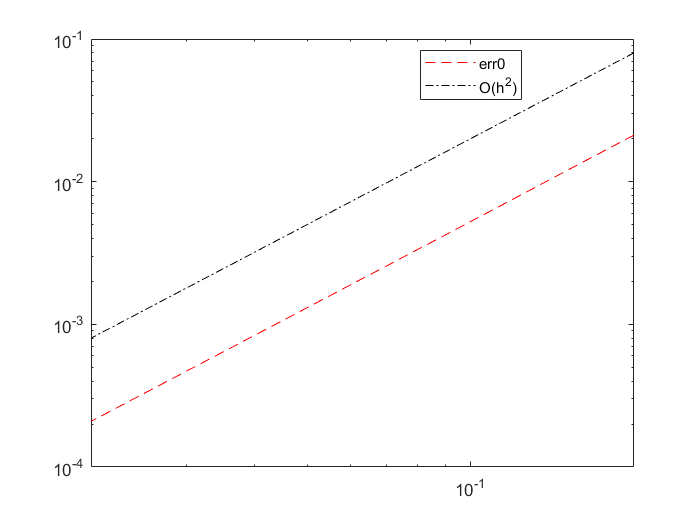
\includegraphics[scale=0.4]{err0_h_1.png}
		\end{minipage}
	}
	\subfigure{
		\begin{minipage}[t]{0.45\linewidth}
			\centering
			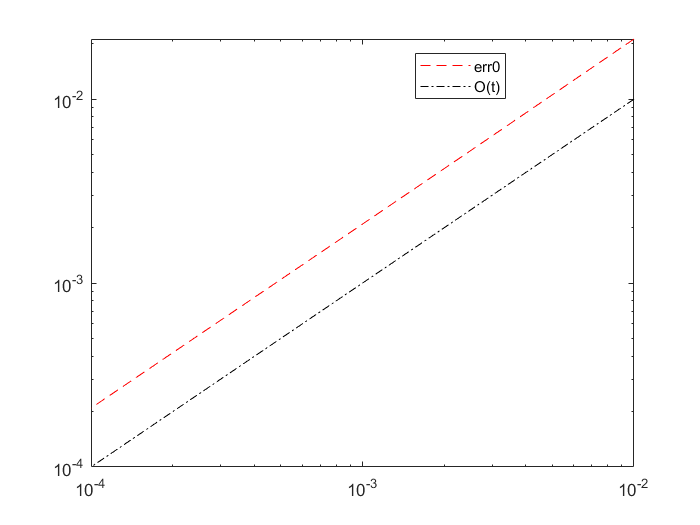
\includegraphics[scale=0.4]{err0_t_1.png}
		\end{minipage}
	}
	\caption{\label{err0} $err0$ 误差的收敛阶}
\end{figure}



%-----------------------------------------------------
\section{实验结果分析}
三种格式的err0 误差关于h的收敛阶均为2,关于t的收敛阶均为1
\end{document}